\section{Diagramas de conexiones}
El siguiente esquema ilustra el circuito fundamental de la experiencia, esquematizando el acoplamiento en paralelo de los devanados primarios y secundarios de los dos transformadores monofásicos.

\begin{figure}[H]
    \centering
    \includegraphics[width=1\linewidth]{imagenes/diagrama 1.png}
    \caption{Esquema de conexión para la operación en paralelo de dos transformadores monofasicos}
    \label{fig:placeholder}
\end{figure}

Con el propósito de validar de las condiciones teóricas indispensables para un acoplamiento seguro, resulto necesario ejecutar ensayos preliminares. Los siguientes diagramas ilustran los montajes experimentales requeridos para evaluar dichos factores críticos antes de proceder con la conexión en paralelo.

\begin{figure}[H]
    \centering
    \includegraphics[width=1\linewidth]{imagenes/Screenshot 2026-10-01 213827.png}
    \caption{Esquema de conexión para deterinar la relación de transformación}
    \label{fig:placeholder}
\end{figure}

\begin{figure}[H]
    \centering
    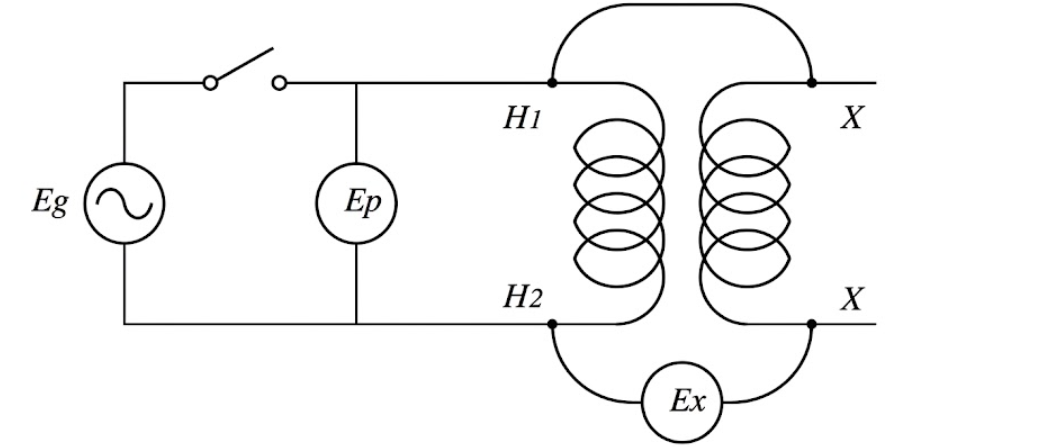
\includegraphics[width=1\linewidth]{IMAGENES/2verdad.png}
    \caption{Esquema de conexión para el ensayo de polaridad}
    \label{fig:placeholder}
\end{figure}

\begin{figure}[H]
    \centering
    \includegraphics[width=1\linewidth]{imagenes/diagrama 3.png}
    \caption{Esquema de conexión para el ensayo de cortocircuito}
    \label{fig:placeholder}
\end{figure}